\documentclass[t]{beamer}

% --- Theme and Color Setup ---
\usetheme{Madrid}
\usepackage{tikz}

% Define the custom Orange color
\definecolor{MyOrange}{RGB}{230, 85, 10} 

% Apply the orange color to the structure
\usecolortheme[named=MyOrange]{structure}

% Fix footer colors to match the orange theme
\setbeamercolor{palette primary}{bg=MyOrange,fg=white}
\setbeamercolor{palette secondary}{bg=MyOrange!80!black,fg=white}
\setbeamercolor{palette tertiary}{bg=MyOrange!60!black,fg=white}
\setbeamerfont{caption}{size=\footnotesize}

% Packages
\usepackage[utf8]{inputenc}
\usepackage{hyperref}
\usepackage{tikz} 
\usepackage{booktabs}
\usepackage{natbib}

% --- 1. CONFIGURATION FOR CONTENT SLIDES (Middle Pages) ---
\addtobeamertemplate{frametitle}{}{%
    \begin{tikzpicture}[remember picture,overlay]
        \node[anchor=north east, xshift=-0.3cm, yshift=0cm, inner sep=0pt] at (current page.north east) {
            % \includegraphics[height=1cm, keepaspectratio]{logo_white.png}
        };
    \end{tikzpicture}%
}

% --- 2. CONFIGURATION FOR FIRST & LAST PAGE ---
\newcommand{\FirstLastPageLayout}{
    \begin{tikzpicture}[remember picture,overlay]
        \node[anchor=north east, xshift=-0.3cm, yshift=0cm, inner sep=0pt] at (current page.north east) {
            % \includegraphics[height=1cm, keepaspectratio]{logo.jpg}
        };
        \node[anchor=south west, xshift=0.5cm, yshift=0.5cm] at (current page.south west) {
            % \textcolor{MyOrange}{\footnotesize Prague University of Economics and Business}
        };
    \end{tikzpicture}
}

% --- Info ---
\title[Title]{\(n+\lvert out \rvert\) vs \(\lvert wcout \rvert\)} % 
% \subtitle{Subtitle of your presentation} % 
\author{Ian Chi} % 
% \institute[]{Department of International Economic Relations} % 
\date{\today}

\begin{document}

% --- Slide 1: Title Page ---
\begin{frame}
    \FirstLastPageLayout % 
    \titlepage
\end{frame}

\begin{frame}
    \frametitle{Yanakakis vs AGM}

    \begin{itemize}
        \item When is Yanakakis faster than AGM?
        \item AGM only cares about shape of hypergraph
        \item Yanakakis is "aware" of the actual relations
    \end{itemize}

\end{frame}

\begin{frame}
    \frametitle{example}
    \begin{columns}
        \begin{column}{0.5\textwidth}
                \begin{itemize}
                    \item fractional edge cover \(= 5\)
                    \begin{itemize}
                        \item AGM guarantees \(O(n^5)\)
                    \end{itemize}
                    \item If \(n=\emptyset\), yanakakis will finish in \(O(n) \)

                \end{itemize}


        \end{column}


        \begin{column}{0.4\textwidth}
            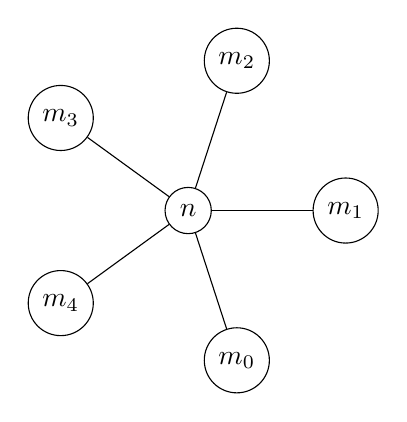
\begin{tikzpicture}[baseline=(current bounding box.north)]
            % Center node
            \node[draw, circle] (C) at (0,0) {$n$};

            % Outer nodes
            \foreach \i in {0,...,4} {
                \node[draw, circle] (N\i) at ({72*(\i-1)}:2.0cm) {$m_\i$};
                \draw (C) -- (N\i);
            }
            \end{tikzpicture}
        \end{column}


    \end{columns}
    
    

\end{frame}



\end{document}